\setcounter{chapter}{15}
\chapter{Critère d'évolution et Piles}

\section{Une transformation est-elle toujours totale ?}
\subsection{Mise en évidence expérimentale}
Nous mettons de l'acide éthanoïque pur dans l'eau et nous obtenons une solution de $\SI{50}{\milli\liter}$ d'acide éthanoïque de concentration $\SI{1,0e-2}{\mole\per\liter}$. Le pH de cette solution est mesuré à 3,4.\\
\small	
\begin{tabular}{|l|p{1.5cm}|p{2cm}|p{1cm}|p{2cm}|p{2cm}|}
\hline 
  \multicolumn{2}{|c!{\protect\makebox[0cm]{:}}}{\textbf{Equation de la réaction}} &
 \multicolumn{1}{c!{\protect\makebox[0cm]{+}}}{%
      $\trou{\rm{CH_3COOH(aq)}}$} &
       \multicolumn{1}{c!{\protect\makebox[0cm]{ $\rightarrow$ }}}{%
      $\trou{\rm{H_2O(l)}}$} 
			&\multicolumn{1}{c!{\protect\makebox[0cm]{ + }}}
			{$\trou{\rm{CH_3COO^-(aq)}}$} 
			&\multicolumn{1}{c|}{
			$\trou{\rm{H_3O^+(aq)}}$} 
\tabularnewline


\hline 
Etat initial&
$x=0$&\trou{\num{5,0e-4}}
&\trou{excès}
&\trou{0}
&\trou{0}

\tabularnewline
\hline 
Etat intermédiaire&
$x$&\trou{\num{5,0e-4}-x}
&\trou{excès}
&\trou{x}
&\trou{x}

\tabularnewline
\hline 
Etat final&
$x=x_{f}$&$\rm \trou{\num{5,0e-4}-x_f}$
&\trou{excès}
&$\rm \trou{x_f}$
&$\rm \trou{x_f}$

\tabularnewline
\hline 
Etat final si tranformation&
$x=x_{max}$&$\trou{\num{5,0e-4}-x_{max}}$
&\trou{excès}
&$\rm \trou{x_{max}}$
&$\rm \trou{x_{max}}$
\tabularnewline
était totale & & & & & 
\tabularnewline
\hline
\end{tabular}\\
\normalsize
\\

Calcul de $\rm x_{max}$\\\trou{$\rm \num{5,0e-4}-x_{max}=0$ donc $\rm x_{max}=\SI{5,0e-4}{\mole}$}\\
Si la réaction était totale, quelle serait la valeur de $\rm x_f$ ?\\
$\rm \trou{x_f=\SI{5,0e-4}{\mole}}$\\
Quelle est la valeur expérimentale de $\rm x_f$ ?\\
\trou{$\rm x_f=[H_3O^+] \times V=10^{-3,4} \times 0,050=\SI{2,0e-5}{\mole}$\\
On remarque que $\rm x_f$ est différent de $\rm x_{max}$, ce qui signifie que la réaction n'est pas totale. Le réactif limitant ne disparaît pas totalement.}

\subsection{Qu'est ce qu'une transformation non totale ?}
\blocgris{Experience}{
Lorsqu'on ajoute à $\SI{50,0}{\milli\liter}$ de la solution d'acide éthanoique de concentration $\SI{1,0e-2}{\mole\per\liter}$ un peu d'ions $\rm CH_3COO^-$ en faisant en sorte que la variation de volume soit négligeable, on constate une augmentation du pH.
}

\etiquette{Interprétation} \\
\trou{On en déduit que $\rm[H_3O^+]$ diminue, ce qui signifie que les ions $\rm H_3O^+$ ont été consommés. Ils ont réagi avec les ions $\rm CH_3COO^-$ selon la réaction $\rm H_3O^++CH_3COO^-\longrightarrow H_2O+CH_3COOH$ }
\\
\trou{Il existe donc deux sens possibles pour la réaction : }
\begin{itemize}
\item \trou{ $\rm CH_3COOH$ réagit avec $\rm H_2O$ pour donner $\rm CH_3COO^-$ et $\rm H_3O^+$}
\item \trou{ $\rm CH_3COO^-$ réagit avec $\rm H_3O^+$ pour donner $\rm CH_3COOH$ et $\rm H_2O$}
\end{itemize}

\trou{La réaction est dite réversible.}
 \trou{
 $H_3O^+ + CH_3COO^- \leftrightharpoons +CH_3COOH$
 }
 \\

Le symbole $\leftrightharpoons$   signifie que la transformation est décrite par deux réactions  \trou{inverses.} On parle d'\textbf{équilibre chimique}.

\subsection{Equilibre dynamique d'un système}
Au niveau microscopique, le système chimique est le siège de deux réactions opposées. Les réactifs réagissent dans le sens \trou{direct} pour former les produits, et les produits réagissent dans le sens \trou{indirect} pour former les réactifs.\\
Au bout d'un moment, il se crée un \trou{équilibre}, et à l'échelle macroscopique, il \textbf{semble} qu'il ne se passe plus rien. 

L'état d'équilibre dynamique du système est alors atteint, et la vitesse de disparition de chaque espèce chimique est égale à sa vitesse d'apparition. Les quantités de matières sont stationnaires: l'équilibre chimique est atteint.
\subsection{Taux d'avancement final}
\blocrouge{Définition}{
Le taux d'avancement final $\tau$ (tau) d'une réaction est défini par le rapport :
\begin{center}
$\tau=\trou{\dfrac{x_f}{x_{max}}}$
\end{center}
}

\blocgris{Exemple}{
Calculer le taux d'avancement final pour la réaction entre l'acide éthanoïque et l'eau décrite au II.1
\\
\trou{$\tau=\dfrac{\SI{2,0e-5}{}}{\SI{5,0e-4}{}}=\SI{4,0e-2}{}$}
\\On constate que $\tau <  1$ ce qui traduit que la réaction n'est pas \texttt{totale}.}

\section{Evolution spontanée d'un système}
\subsection{Définition de l'activité}
L'activité d'une espèce chimique X se note $\alpha(X)$. C'est une grandeur sans dimension.\\
\begin{itemize}
\item Si X est une espèce en solution, alors $\alpha(X)=\dfrac{[X]}{c^0}$ avec $c^0=\SI{1}{\mole\per\liter}$
\item Si X est le solvant, alors $\alpha(X)=1$. Ce qui est très souvent le cas de l'eau.
\item Si X est une espèce solide, alors  $\alpha(X)=1$.
\end{itemize}

% suite

 \etiquette{Exemple}
 Exprimer l'activité de chaque espèce présente dans l'équation de la réaction de l'acide éthanoïque avec l'eau :\\
 \trou{$\alpha(CH_3COOH)=\dfrac{[CH_3COOH]}{c^0}$\\
 $\alpha(H_2O)=1$\\
$\alpha(CH_3COO^-)=\dfrac{[CH_3COO^-]}{c^0}$\\
$\alpha(H_3O^+)=\dfrac{[H_3O^+]}{c^0}$}

\subsection{Quotient de réaction}
\blocrouge{Définition}{
Considérons une réaction de la forme :$$aA + bB \leftrightharpoons cC +dD$$
 $Q_r$,  quotient de réaction est défini comme étant le produit :\\
 \begin{center}$Q_r=\trou{\dfrac{\alpha(C)^c\alpha(D)^d}{\alpha(A)^a\alpha(B)^b}}$\end{center}
 $Q_r$ est une grandeur sans unité.}

 \etiquette{Exemple} \\
 Exprimer le quotient de réaction dans le cas de la réaction de l'acide éthanoïque avec l'eau :\\
 \trou{$Q_r=\dfrac{\alpha(H_3O^+)\alpha(CH_3COO^-)}{\alpha(CH_3COOH)}=\dfrac{\dfrac{[H_3O^+]}{c^0}\dfrac{[CH_3COO^-]}{c^0}}{\dfrac{[CH_3COOH]}{c^0}}=\dfrac{[H_3O^+][CH_3COO^-]}{[CH_3COOH]c^0}$}


\subsection{Constante d'équilibre}
\blocrouge{Définition}{Lorsque le système chimique a atteint l'état d'équilibre, la valeur du quotient réactionnel est appelée: \trou{constante d'équilibre}. Elle se note K. $$\trou{Q_{r(eq)}= K}$$}
%\blocgris{Activité introductive}{
%On considère la réaction d'estérification, lors de laquelle un alcool réagit avec un acide pour donner un ester et de l'eau.\\
%La réaction étudiée fait réagir l'éthanol et l'acide éthanoïque. L'ester obtenu est l'éthanoate d'éthyle.\\
%L'équation de la réaction s'écrit : 
%$$CH_2CH_3OH + CH_3COOH\leftrightharpoons H_2O +CH_3COOCH_2CH_3$$
%
%\textbf{Cas \no1} : $n_i(alcool)=\SI{1,0}{\mole}$ ; $n_i(acide)=\SI{1,0}{\mole}$. \\ On obtient alors, à l'état final : $n_f(ester)=\SI{0,67}{\mole}$ ; $n_f(eau)=\SI{0,67}{\mole}$.\\
%\textbf{Cas \no2} : $n_i(alcool)=\SI{1,0}{\mole}$ ; $n_i(acide)=\SI{5,0}{\mole}$. \\ On obtient alors, à l'état final : $n_f(ester)=\SI{0,946}{\mole}$ ; $n_f(eau)=\SI{0,946}{\mole}$.\\
%\textbf{Cas \no3} : $n_i(alcool)=\SI{1,0}{\mole}$ ; $n_i(acide)=\SI{2,0}{\mole}$. \\ On obtient alors, à l'état final : $n_f(ester)=\SI{0,848}{\mole}$ ; $n_f(eau)=\SI{0,848}{\mole}$.\\
%Remarque : ici, l'eau n'est pas le solvant, on la prend donc en compte dans le calcul du quotient de réaction.\\
%Pour chaque cas, calculer le quotient de réaction à l'équilibre. Que remarquez-vous ?
%}

% suite

\etiquetterouge{Propriétés de K}
\begin{itemize}
	\item K ne dépend que de la \trou{température} mais pas de l'état initial du système.
	\item Pour la réaction d'un acide dans l'eau, K s'appelle la constante \trou{d'acidité} et se note Ka. 	
\end{itemize}



 \blocgris{Exemple}{
 Donner l'expression de la constante d'équilibre dans le cas de la réaction de l'acide éthanoïque avec l'eau (page 1) puis calculer sa valeur.\\ On rappelle que $[H_3O^+]_{eq}=\SI{3.98e-4}{\mol\per\liter}=[CH_3COO^-]_{eq}$ et  $[CH_3COOH]_{eq}=\SI{9.60e-3}{\mol\per\liter}$\\
 \trou{$K=\dfrac{\dfrac{[H_3O^+]_{eq}}{c^0}\dfrac{[CH_3COO^-]_{eq}}{c^0}}{\dfrac{[CH_3COOH]_{eq}}{c^0}}=\dfrac{[H_3O^+]_{eq}[CH_3COO^-]_{eq}}{[CH_3COOH]_{eq}c^0}$}\\
 \trou{$K=\dfrac{(10^{-3,4})^2}{\dfrac{\SI{5,0e-4}{}}{\SI{50e-3}{}}-10^{-3,4}}=\SI{1,65e-5}{}$}
 }
 \newpage
\subsection{Prévision du sens d'évolution}
%Reprenons l'exemple de la réaction d'estérification. 
%La réaction s'écrit : \\
%\begin{center}
%$$CH_2CH_3OH + CH_3COOH\leftrightharpoons H_2O +CH_3COOCH_2CH_3$$
%\end{center}
%L'acide est le réactif limitant. Au bout d'un certain temps, l'équilibre est atteint et le système n'évolue plus.\\
%Écrire le quotient de réaction à l'équilibre en notant $[ester]_{eq}$, $[acide]_{eq}$, $[alcool]_{eq}$ et $[eau]_{eq}$ les concentrations à l'équilibre.\\
%\begin{center}
%\trou{$Q_r=\dfrac{[ester]_{eq}[eau]_{eq}}{[acide]_{eq}[alcool]_{eq}}$}\\
%\end{center}
%Que pourrait-on faire pour que la réaction reparte dans le sens \no 1 ? \\
%\trou{On retire de l'eau. \\
%  Si [eau] diminue, on remarque que $Q_r$ diminue et la réaction évolue alors dans le sens 1.\\
%  On ajoute du réactif de l'alcool, réactif non limitant.\\
%  Si [alcool] augmente, on remarque que $Q_r$ diminue et la réaction évolue alors dans le sens 1.}
%  
  %
\etiquetterouge{Critères d'évolution}

On dispose d'un système chimique dont on connaît les concentrations initiales. On calcule le quotient réactionnel\textbf{ initial}: \trou{$Q_{ri}$}. On le compare à la constante d'équilibre K.
Il y a 3 cas à envisager: 

\begin{minipage}{0,58\linewidth}
\begin{enumerate}
\item Si $Q_r<K$, alors le système est hors équilibre et évolue dans le sens \trou{direct}.
\item Si $Q_r>K$, alors le système est hors équilibre et évolue dans le sens \trou{indirect}.
\item Si $Q_r=K$, alors le système a atteint son équilibre, et il \trou{n'évolue plus}.
\end{enumerate}
\end{minipage}
\begin{minipage}{0,40\linewidth}
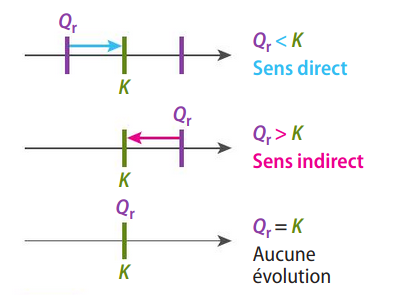
\includegraphics[scale=0.58]{figures/evolution/fig_K}
\end{minipage}

\etiquette{Exercice} 10 p 145 (important) 9 p 145



\newpage
\section{La pile, un transfert d'électrons}
\subsection{Un exemple de réaction d'oxydo-réduction}
\subsection*{Expérience}

\begin{figure}[h]
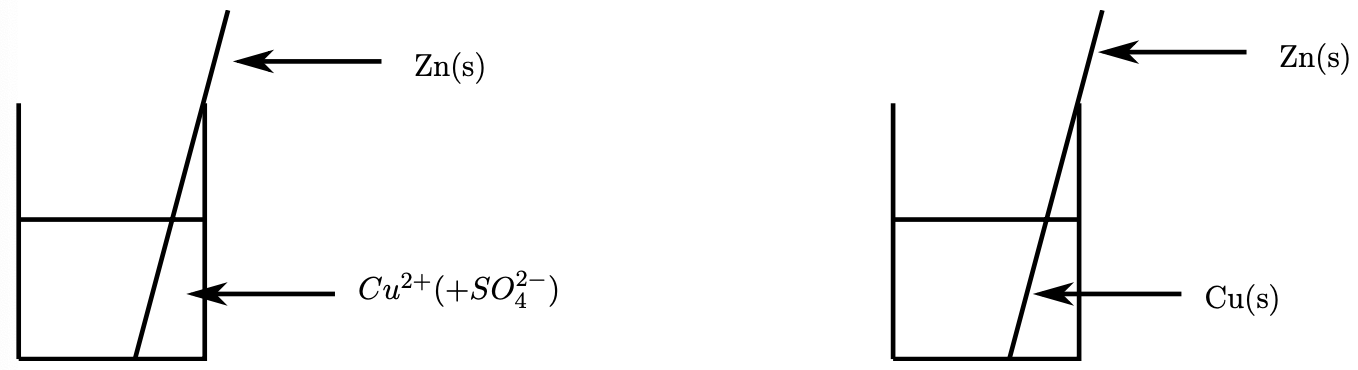
\includegraphics[scale=0.45]{figures/evolution/pile}
\end{figure}

\subsection*{Interprétation :}
On observe l'apparition de \trou{cuivre} sur la plaque de zinc. La réaction qui a eu lieu est donc :\\
\trou{$Cu^{2+}(aq) + 2e-=Cu(s)$}\\
D'où ces deux électrons peuvent-ils venir ?
Les deux électrons ont été cédés par \trou{le zinc : $Zn(s)=Zn^{2+}(aq) + 2e-$}\\
\trou{Donc, les deux électrons cédés par le zinc ont été captés par les ions $Cu^{2+}$}\\
On obtient donc l'équation de la réaction suivante :\\
\trou{$Zn(s)+Cu^{2+}(aq) \longrightarrow Zn^{2+}(aq) + Cu(s)$}


\etiquetterouge{Remarque} Cette réaction a eu lieu spontanément ce qui signifie qu'à l'état initial $Q_{ri}< K$. Vérifiez-le.

\subsection{Détournement d'électrons, réalisation d'une pile}
\etiquette{Montage expérimental} Pour réaliser une pile, on utilise de demi-pile. Un demi-pile est formée par l'association d'un métal et d'une solution contenant l'ion métallique.
\begin{center}
\begin{figure}[htp!]
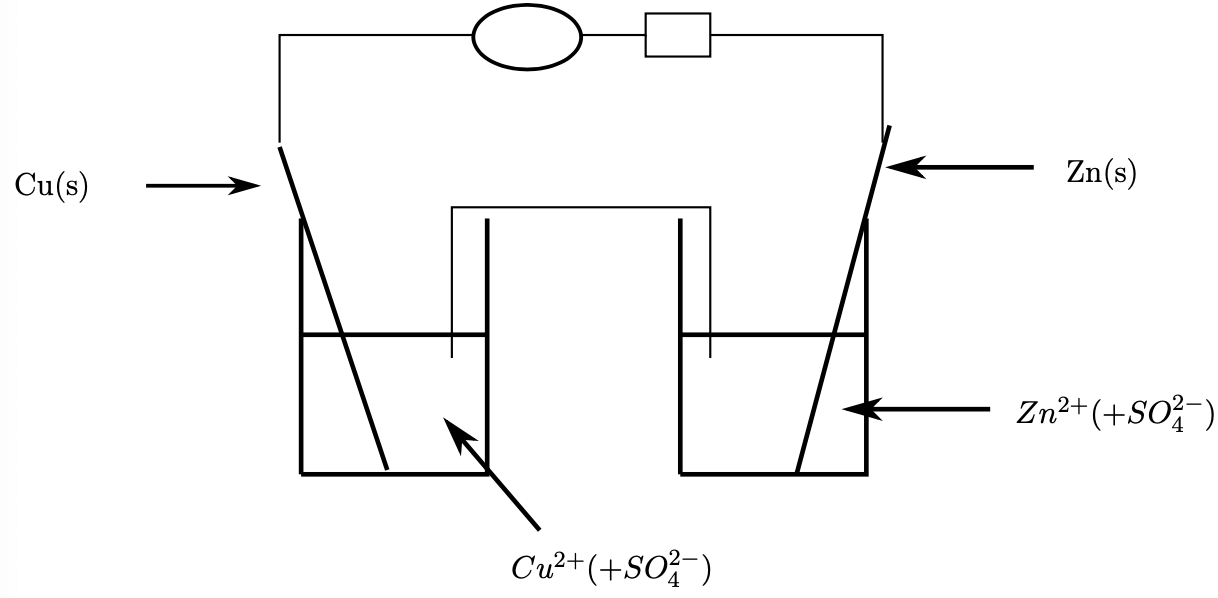
\includegraphics[scale=0.5]{figures/evolution/pile1}
\end{figure}
  \end{center}

\subsection*{Observations}

A l'aide d'un ampèremètre, on constate  \trou{qu'un courant circule de la lame de cuivre vers la lame de zinc à l'extérieur de la pile.}

\etiquette{Questions à se poser}

\begin{itemize}
	\item Où est le pôle positif ? le pôle négatif ?
	\item Quel est le sens de déplacement des électrons ? Celui du sens conventionnel du courant ? Les représenter sur le schéma de la pile.
	\item Les électrons se déplacent-ils dans les solutions ?
	\item Sachant que \textbf{l'oxydation} a \textbf{toujours} lieu à l\trou{'\textbf{anode}}. A quel pôle de la pile se situe l'anode ?
	\item Même travail pour la \textbf{cathode}.
\end{itemize}

\etiquetterouge{Fonctionnement de la pile}

Lorsque les électrons créés par la réaction d'\trou{oxydation} du zinc arrivent au niveau de la lame de cuivre, ils sont captés par les ions cuivre II pour former du cuivre. Les électrons sont forcés à circuler à l'\trou{extérieur} de la pile, ce qui génère un\trou{ courant électrique}, voilà pourquoi on peut évoquer un détournement d'électrons.

\subsection*{Équation globale de la pile} Lorsque la pile fonctionne (débite du \trou{courant}) cela se traduit par la réaction d'équation: 
$$Zn(s)+Cu^{2+}(aq) \longrightarrow \trou{Zn^{2+}(aq)+Cu(s)}$$

\subsection*{Rôle du pont salin}
Le pont salin assure la \trou{fermeture du circuit} électrique. Il est constitué d'un papier imbibé d'une solution contenant des ions (par exemple: $K^+ + NO_3^-$)\\
Il n'y a pas d'électron dans le pont salin puisque les électrons ne se trouvent jamais en solution. Ce sont les ions qui conduisent le courant en solution.

\etiquette{Travail}
Compléter sur le schéma le sens de déplacement des ions dans le pont salin.

\subsection*{Tension à vide ou f.e.m (force électromotrice)}
\begin{minipage}{0,6\linewidth}
La tension mesurée aux bornes de la pile lorsqu'elle ne débite pas est appelée \trou{tension à vide}. Elle est exprimée en volts.\\
Sur le schéma ci-contre, la borne V définit la borne positive de la pile
\end{minipage}
\begin{minipage}{0,4\linewidth}
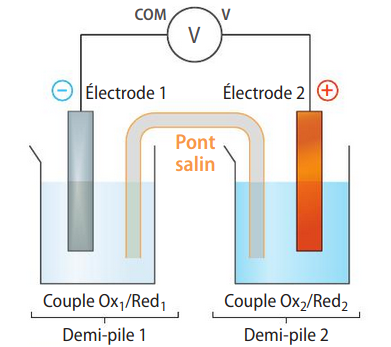
\includegraphics[scale=0.5]{figures/evolution/pile3}
\end{minipage}


\etiquetterouge{Important} Qu'est-ce qu'une pile usée ?\\
La pile en fonctionnement est un système hors \trou{ équilibre}, lorsqu'elle atteint \textbf{l'équilibre}, la réaction \trou{s'arrête}, le courant ne circule plus, la pile est \trou{\textbf{usée}}.

\subsection{Capacité d'une pile}
\blocrouge{Définition}{La capacité d'une pile, notée Q, est égale à la \trou{charge électrique} qui circule pendant la durée totale de son fonctionnement, de l'état initial à l'usure complète. La capacité de la pile s'exprime \trou{coulomb (C)}. \\ Rien à voir avec le quotient réactionnel Qr !!
}

Si l'on considère que l'intensité du courant I est constante pendant toute la durée de fonctionnement, alors on a :
$$\boxed{Q=\trou{I\times \Delta t}}$$
\begin{center}
 avec 
Q la capacité de la pile en coulombs(C)\\
I l'intensité du courant en ampères (A)\\
$\Delta t$ le durée de vie de la pile en secondes (s)
\end{center}
On peut également calculer la capacité d'une pile grâce à l'expression :$$\boxed{Q=\trou{n(e^-) \times F}}$$
\begin{itemize}
	\item $n(e^-)$ le nombre d'électrons échangés pendant le fonctionnement.
	\item F la constante de faraday : $F=e\times N_a=\SI{9,65e4}{\coulomb\per\mole}$ C'est la charge d'une mole d'électrons.

\end{itemize}
%\newpage
\etiquette{Exercices sur les piles}
\begin{itemize}
	\item 14 
	\item  16
	\item  19
	\item  28 p 146
\end{itemize}

Type bac: \url{https://www.labolycee.org/defibrillateur-cardiaque-implantable}
%
%
%\section{Electrolyse}
%\subsection{Transformation forcée}
%\etiquetterouge{Idée forte} En apportant de l'énergie électrique à un système chimique, il est possible de\trou{ renverser }le sens de l'évolution spontané d'une réaction chimique, c'est \textbf{\trou{l'électrolyse}}. L'énergie est apporté par un \textbf{générateur} qui va \textbf{\trou{imposer le sens }du courant} et donc celui des échanges d'électrons.
%
%\subsection{Electrolyse d'une solution de chlorure d'étain}
%\etiquette{Montage}
%
%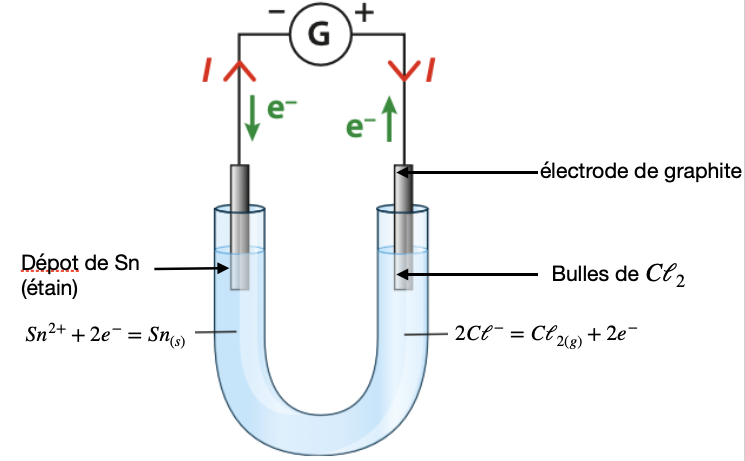
\includegraphics[width=12 cm]{figures/electrolyse_3}
%
%Vidéo de l'expérience: \url{https://www.youtube.com/watch?v=0KI65y_b5y4}
%
%\subsection{Obtention des équations redox}
%
%On sait que :
%\begin{itemize}
%	\item Le courant I et le sens des $e^-$ est imposé par le générateur. 
%	\item Initialement les seules espèces chimiques présentes sont: $C\ell^-$ et $Sn^{2+}$.
%	\item Les couples sont $C\ell_{2(g)} / C\ell^-$ et $Sn^{2+} / Sn$.
%	\item Equations redox des couples $$\trou{C\ell_{2(g)}} + 2e^- = \trou{C\ell^-}$$ $$Sn^{2+}+\trou{2e^-}=\trou{Sn}$$
%\end{itemize}
% On en déduit que: 
%\begin{itemize}
%	\item Les électrons arrivent à gauche. Il sont consommés selon $$\trou{Sn^{2+}}+2e^- = \trou{Sn}$$
%	\item Les électrons qui partent de l'électrode à droite sont produits par $$2C\ell^-=C\ell_{2(g)}+\trou{2e^-}$$
%\end{itemize}
%
%\subsection{Interprétation chimique}
%
%Durant l'électrolyse, on observe la réaction d'équation $$\trou{2C\ell^-+Sn^{2+}}\longrightarrow \trou{C\ell_{2(g)}+Sn_{(s)}}$$ 
%
%\blocgris{Questions}{
%On donne:  l'activité initiale du dichlore vaut 1, $[Sn^{2+}]_i = 0,5$ mol/L et $[C\ell^-]_i = 1$ mol/L.
%\begin{enumerate}
%	\item Quelle est la valeur de $Q_{ri}$ ? 
%	\item Sachant que K = \num{e-51}. Quelle est le sens spontanée de la réaction chimique.
%	\item Justifier qu'il s'agit ici d'une réaction forcée.
%\end{enumerate}
%}
%\section{Quelques couples oxydant-réducteur usuels}
%\blocgris{Demi-équations}{
%Pour chacun des couples ci-dessous, écrire la demi-équation d'oxydo-réduction : 
%\begin{itemize}
%\item L'eau de javel est une solution d'ion hypochlorite $ClO^-$ oxydant du couple : $ClO^-/Cl^-$\\
%\trou{$ClO^-+H_20+2e-=Cl^-+2HO^-$}
%\item le dioxygène $O_2$ est l'oxydant du couple $O_2/H_2O$\\
%\trou{$O_2+4e-+4H^+=2H_2O$}
%\item le dichlore $Cl_2$ est l'oxydant du couple $Cl_2/Cl^-$\\
%\trou{$Cl_2+2e-=2Cl^-$}
%\item l'acide ascorbique ou vitamine C est le réducteur du couple $C_6H_6O_6/C_6H_8O_6$\\
%\trou{$C_6H_6O_6 +2H^+  = C_6H_8O_6$}
%\item le dihydrogène $H_2$ est le réducteur du couple $H^+/H_2$.\\
%\trou{$2H^+ +2e-=H_2$}
%\end{itemize}
%}
%\etiquette{Remarque}
%Les éléments des deux premières colonnes du tableau périodique sont les éléments du bloc s. Ils ont tous un ou deux électrons sur leur couche externe. Ils sont donc susceptibles de les perdre, ce qui fait d'eau des \trou{réducteurs}
%
%\etiquette{Récap du cours sur électrolyse} \url{https://www.youtube.com/watch?v=w3lg9HDBMKw}
%
%
%\etiquette{Exercices sur l'électrolyse}
%1, 2, 8, 12 et 18 p 184
%type bac: \url{https://www.labolycee.org/corrosion-et-protection-des-metaux}
